% Figure 4 -- (a) n-2 bifundamentals between two U(1)'s; (b) leg of the regular singularity;
%             (c) U(2) split into two U(1)'s; (d) the glued quiver
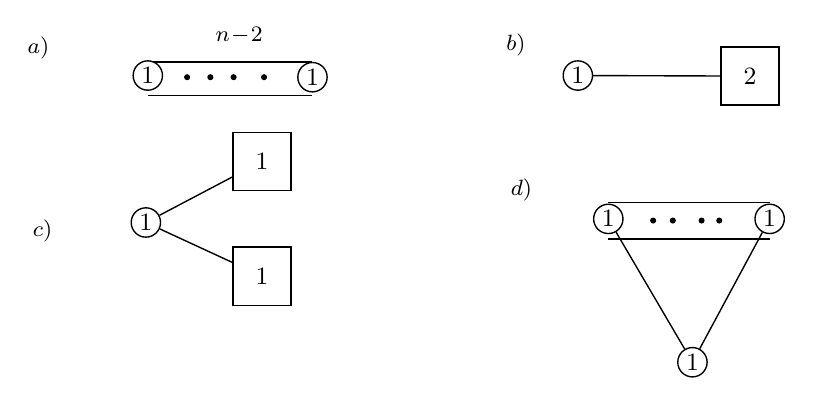
\begin{tikzpicture}[x=1pt,y=1pt,>=stealth,line width=0.5pt,
    nd/.style={circle,draw,fill=white,inner sep=0pt,minimum size=10.6pt,font=\small},
    sq/.style={rectangle,draw,fill=white,inner sep=0pt,minimum size=21pt,font=\small}]
  % ---------------- a) ----------------
  \draw (53,120.4) -- (112.5,120.4);
  \draw (53,108.35) -- (112.5,108.35);
  \node[nd] (a1) at (53,115.5) {1};
  \node[nd] (a2) at (112.5,114.9) {1};
  \foreach \x in {67.2,75.6,84.0,95.0} {\fill (\x,114.9) circle[radius=1.1pt];}
  \node[inner sep=0pt,font=\footnotesize] at (86,129.8) {$n\!-\!2$};
  \node[inner sep=0pt,font=\footnotesize] at (13.5,125.3) {$a)$};
  % ---------------- b) ----------------
  \node[nd] (b1) at (208.4,115.5) {1};
  \node[sq] (b2) at (270.6,115.3) {2};
  \draw (b1) -- (b2);
  \node[inner sep=0pt,font=\footnotesize] at (186,126.6) {$b)$};
  % ---------------- c) ----------------
  \node[nd] (c1) at (52.3,62.4) {1};
  \node[sq] (c2) at (94.3,43.0) {1};
  \node[sq] (c3) at (94.3,84.5) {1};
  \draw (c1) -- (c2);
  \draw (c1) -- (c3);
  \node[inner sep=0pt,font=\footnotesize] at (15,59.2) {$c)$};
  % ---------------- d) ----------------
  \draw (219.4,69.6) -- (277.7,69.6);
  \draw (219.4,56.5) -- (277.7,56.5);
  \node[nd] (d1) at (219.4,63.7) {1};
  \node[nd] (d2) at (277.7,63.7) {1};
  \node[nd] (d3) at (249.8,11.9) {1};
  \draw (d1) -- (d3);
  \draw (d2) -- (d3);
  \foreach \x in {235.6,242.7,253.1,259.5} {\fill (\x,63.1) circle[radius=1.1pt];}
  \node[inner sep=0pt,font=\footnotesize] at (188,74.1) {$d)$};
\end{tikzpicture}
